\chapter{A kiberbiztonsági analízis metodológiája}

A diplomamunkám legfontosabb része a metodológia előállítása volt. A metodológia az ami biztosítja azoknak a céloknak az elérését, hogy az analízis (i) teljes körű legyen, (ii) megismételhető legyen és (iii) már létező információkra építsen, azon túl, hogy az eredménye és használata minél átláthatóbb legyen a stakeholderek és az elemző mérnök számára is.

Ez a metodológia kapcsolja össze az autóiparra jellemző rendszermodelleket a fenyegetésmodellekkel. Ennek segítségére és támogatására készült el a kapcsolódó modellező eszköz és ennek az eredménye az egyik legfontosabb előállított értéke a kiberbiztonsági mérnök feladatkörnek.

Az \textit{Áttekintés} fejezet tartalmaz egy magas szintű végigvezetést a bemenetektől a kimenetig és a közte megtett lépésekről.

A \textit{Termékleírás és fenyegetésmodell származtatása} mutatja be a kiindulómodell elkészítésének lépéseit valamint, hogy abból, hogyan állítjuk elő a fenyegetés modellt.

A \textit{Fenyegetésmodellezés} fejezetben láthatóak a további lépések a fenyegetésmodell specifikálására, valamint be mutatja a fenyegetésmodellből előállított támadási fák konstrukcióját és annak szerkesztésének lépéseit.

A \textit{Dokumentumok generálása és manuális analízis} fejezetben pedig találhatóak a szabvány által előírt output előállítása és az elemző eszköz használatát követő folyamatok.

\section{Áttekintés}

A metodológiám fő feladata a \textit{Háttérismeretek} fejezetben található \textit{Követelmények a fenyegetéselemzésre és kockázatértékelésre} részben leírtakat követve kialakítsam azt a lépéssorozatot amelyet az általam fejlesztett eszköz támogatásával végre lehet hajtani és el lehet jutni egy általános autóipari modellből a kockázatelemzés eredményéig.

A lépésekről egy áttekintés a \ref{fig:04_OVERVIEW} ábrán látható. Itt egyrészről a fehér hátterű négyzetekben az ISO 21434 által definiált lépések láthatóak amelyek bővebb leírása a \textit{Háttérismeretek} részben található, lila hátterű négyzetekben pedig az ebben a fejezetben bemutatott lépések láthatóak. Így látható egy egyszerűbb áttekintés a két módszertan közti fedettségről.

\begin{figure}[!ht]
	\centering
	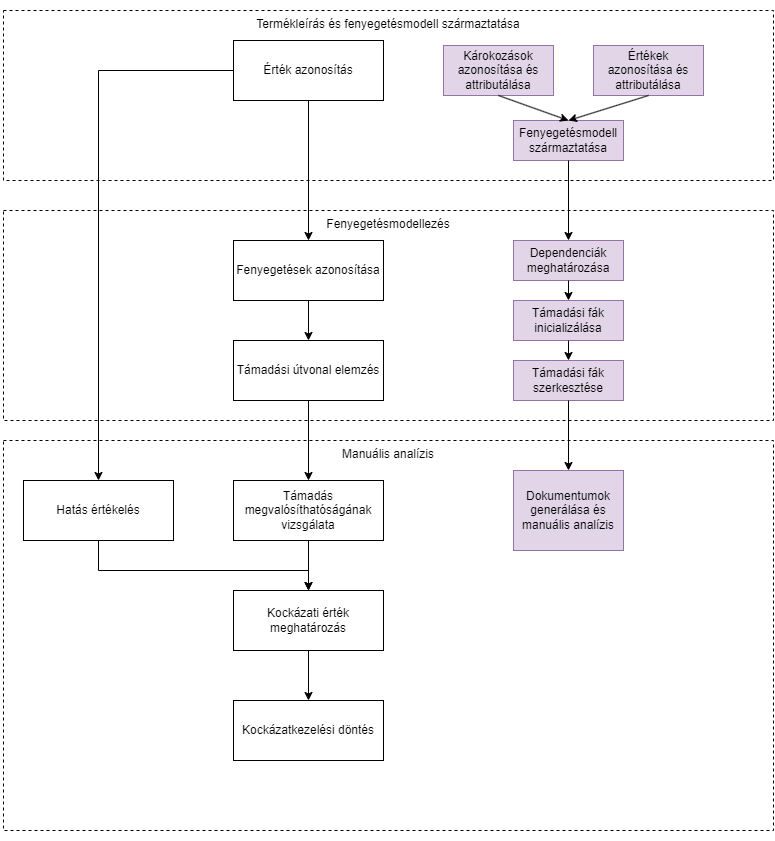
\includegraphics[width=130mm, keepaspectratio]{figures/04_overview.png}
	\caption{Metodológia áttekintése}
	\label{fig:04_OVERVIEW}
\end{figure}

\section{Termékleírás és fenyegetésmodell származtatása}

Ez a fejezet mutatja be az első lépéseit a kockázatelemzési folyamatnak. Itt lesz szükségünk a kiinduláskor rendelkezésünkre álló termékleírást (ami a rendszermodell egy részhalmaza) bővíteni kiberbiztonsági attribútumokkal majd abból származtatni egy olyan új modellt ami a kiberbiztonsági elemzésre alkalmas lesz.

\subsection{Károkozások azonosítása és attributálása}



\subsection{Értékek azonosítása és attributálása}

\subsection{Fenyegetésmodell származtatása}

\section{Fenyegetésmodellezés}

\subsection{Dependenciák meghatározása}

\subsection{Támadási fák inicializálása}

\subsection{Támadási fák szerkesztése}

\section{Dokumentumok generálása és manuális analízis}